\setcounter{section}{1}
\section{Modellierung von dynamischen Systemen}
\begin{tcolorbox}[colback=white!10!white,
                  colframe=blue!50!black,
                  title=KOCHREZEPT: Freischneiden]
    Massen $\{m_1,\hdots,m_n\}$ mit $\{x_1,\hdots,x_m\}$ \\
    Anfangsbedingung: $x_1 = \hdots = x_m = 0$ \\\\
    \begin{minipage}{0.3\textwidth}
        \centering
        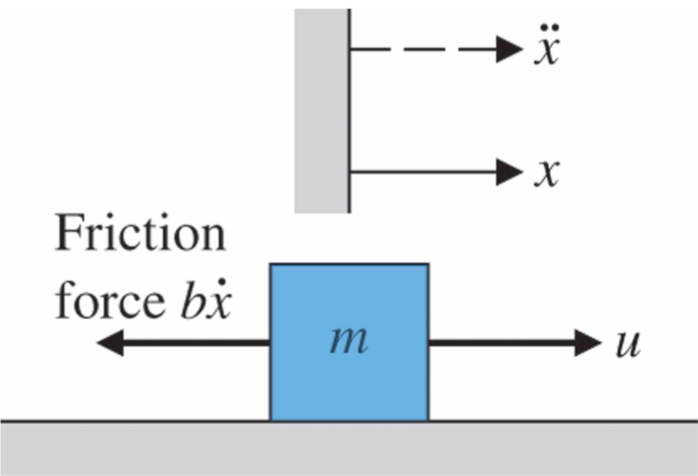
\includegraphics[width=\textwidth]{images/free_body_diagram}
    \end{minipage}
    %\hspace{0.05\textwidth}
    \begin{minipage}{0.65\textwidth}
        \begin{enumerate}
            \item Freischneiden: $\forall{x_i}\forall{x_j}: x_j \neq x_i :$ \\
                $x_j$ ,,festhalten'', \\
                $x_i$ ,,erhöhen'' und Pfeile entgegengesetzt ausrichten, so dass
                \begin{itemize}
                    \item $\forall k: k(x_i - x_j)$
                    \item $\forall b: b(\dot{x}_i - \dot{x}_j)$
                \end{itemize}
            \item Gleichungssystem: \\
                $\sum F = 0 = m_i \ddot{x}_i$ \\
                Vorzeichen aller entgegengesetzten Kräfte sind negativ.
            \item Stabilität: \\
                System ist stabil, sobald mindestens eine $m_i$ unabhängig 
                gedämpft oder das System nur einseitig beschränkt ist.
        \end{enumerate}
    \end{minipage}
\end{tcolorbox}

\begin{tcolorbox}[colback=white!10!white,
                  colframe=gray!50!black,
                  title=Beispiel]
    \begin{minipage}{0.3\textwidth}
        Aufgabe:
        \centering
        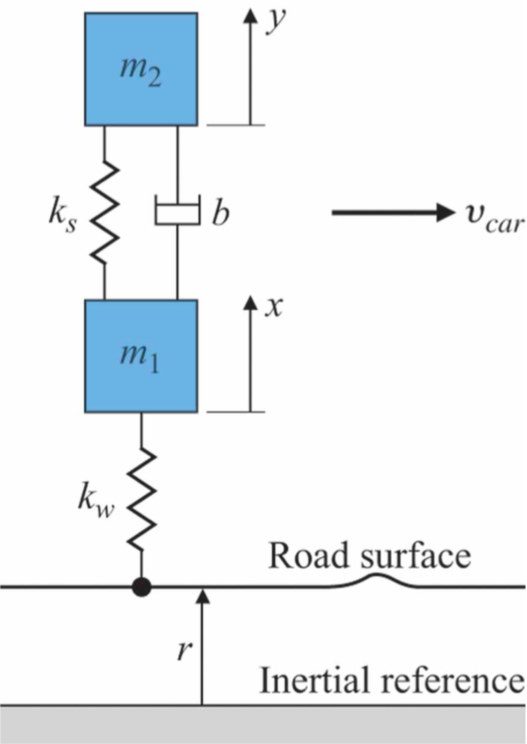
\includegraphics[width=\textwidth]{images/free_body_diag_example1_a}
    \end{minipage}
    \begin{minipage}{0.65\textwidth}
        Freigeschnitten:
        \centering
        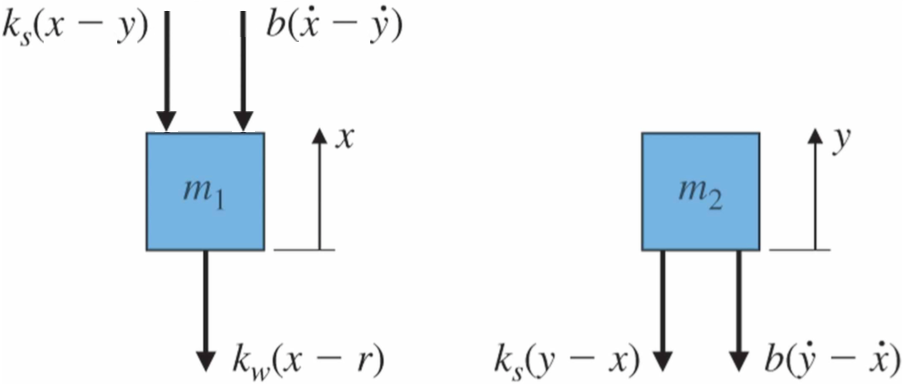
\includegraphics[width=\textwidth]{images/free_body_diag_example1_b}
    \end{minipage}
    Gleichungssystem:
    \begin{equation*}\begin{matrix}
        m_1 \cdot \ddot{x} & = & -k_w(x-r) - k_s(x-y) - b(\dot{x}-\dot{y}) \\
        m_2 \cdot \ddot{y} & = & -k_s(y-x) - b(\dot{y}-\dot{x}) \\\\
        \frac{k_w}{m_1} r & =
            & \ddot{x} + \frac{b}{m_1} \dot{x} + \frac{k_w+k_s}{m_1} x
            - \frac{b}{m_1} \dot{y} - \frac{k_s}{m_1} y \\ 
        0 & = & \ddot{y} + \frac{b}{m_2} \dot{y} + \frac{k_s}{m_2} y
            - \frac{b}{m_2} \dot{x} - \frac{k_s}{m_2} x \\\\
        \frac{k_w}{m_1} R(s) & =
            & \Bigl( s^2 + s\frac{b}{m_1} + \frac{k_w+k_s}{m_1} \Bigr) X(s)
            - \Bigl(s\frac{b}{m_1} + \frac{k_s}{m_1} \Bigr) Y(s) \\ 
        0 & = & \Bigl( s^2 + s\frac{b}{m_2} + \frac{k_s}{m_2} \Bigr) Y(s)
            - \Bigl( s\frac{b}{m_2} + \frac{k_s}{m_2} \Bigr) X(s) \\\\
    \end{matrix}\end{equation*}
\end{tcolorbox}